
\section{Experiment 1: Pointing Correction Model}
In this section, we present the results obtained from the second experiment.
Prior to presenting the results, we provide a reminder of the RMS ratio measure \eqref{eq:mean_rms_compared}, which will be frequently used in this section.
This measure is used to compare the current pointing model to the machine learning model, and a value less than $1$ indicates an improvement of the current model. \\

Table \ref{tab:results_minval_val_test_days_04_n230} presents the validation and test RMS ratios for all folds of the NFLASH230 model in case 1 and case 2.
Recall that models were trained with different numbers of features $k$, and these results are from the model with the best performance on the validation set.
The results show that the model's performance on the validation set is very good in both case 1 and 2.
However, this does not generalize well to the test set, with the performance on the test set for case 1 being significantly worse than the current model for all folds.
In contrast, for case 2, the performance on the test set is better than the current model for most of the folds.
Table \ref{tab:results_minval_val_test_days_04_all} presents the same results for the model predicting the offsets of all instruments.
This model exhibits similar trends, although its performance on the test set is not as good as the NFLASH230 model.\\

\begin{table}[!htbp]
    \centering
    \caption{Validation and test performance for Case 1 and 2, only NFLASH230.
    Performance when choosing the model complexity that yields the best results on the validation set for the given fold.}
    \begin{tabular}{lccccc}
        \toprule
        & & \multicolumn{2}{c}{Case 1 RMS ratio} & \multicolumn{2}{c}{Case 2 RMS ratio} \\
        \cmidrule{3-4} \cmidrule{5-6}
        Target & Fold & Validation & Test &  Validaiton &  Test \\
        \midrule
        \multirow{6}{*}{Azimuth} & 1 &  0.848 &       1.188 &      0.846 &       1.043 \\
                            & 2 &  0.841 &       1.427 &      0.870 &       0.962 \\
                            & 3 &  0.840 &       1.462 &      0.923 &       0.882 \\
                            & 4 &  0.837 &       1.266 &      0.873 &       0.989 \\
                            & 5 &  0.846 &       1.242 &      0.879 &       0.944 \\
                            & 6 &  0.837 &       1.318 &      0.907 &       0.930 \\
        \hline
        \multirow{6}{*}{Elevation} & 1 &  0.835 &       1.173 &      0.887 &       1.030 \\
                            & 2 &  0.831 &       1.188 &      0.889 &       0.973 \\
                            & 3 &  0.831 &       1.204 &      0.886 &       1.025 \\
                            & 4 &  0.812 &       1.198 &      0.826 &       0.844 \\
                            & 5 &  0.815 &       1.166 &      0.802 &       0.870 \\
                            & 6 &  0.810 &       1.262 &      0.825 &       0.906 \\
        \bottomrule
    \end{tabular}
    \label{tab:results_minval_val_test_days_04_n230}
\end{table}

\newpage 
\begin{table}[!htbp]
    \centering
    \caption{Validation and test performance for Case 1 and 2, all instruments.
    Performance when choosing the model complexity that yields the best results on the validation set for the given fold.}
    \begin{tabular}{lccccc}
        \toprule
        & & \multicolumn{2}{c}{Case 1 RMS ratio} & \multicolumn{2}{c}{Case 2 RMS ratio} \\
        \cmidrule{3-4} \cmidrule{5-6}
        Target & Fold & Validation & Test &  Validaiton &  Test \\
        \midrule
        \multirow{6}{*}{Azimuth} & 1 &  0.870 &       1.642 &      0.881 &       1.233 \\
                            & 2 &  0.861 &       1.626 &      0.971 &       0.928 \\
                            & 3 &  0.876 &       1.784 &      0.897 &       1.016 \\
                            & 4 &  0.866 &       1.613 &      0.938 &       0.950 \\
                            & 5 &  0.862 &       1.935 &      0.927 &       0.942 \\
                            & 6 &  0.874 &       1.779 &      0.923 &       1.027 \\
                            \hline
        \multirow{6}{*}{Elevation} & 1 &  0.832 &       1.193 &      0.948 &       0.965 \\
                            & 2 &  0.831 &       1.141 &      0.924 &       1.051 \\
                            & 3 &  0.824 &       1.129 &      0.929 &       1.094 \\
                            & 4 &  0.816 &       1.172 &      0.822 &       0.922 \\
                            & 5 &  0.818 &       1.196 &      0.828 &       0.978 \\
                            & 6 &  0.822 &       1.186 &      0.831 &       0.951 \\
                            \bottomrule
    \end{tabular}
    \label{tab:results_minval_val_test_days_04_all}
\end{table}


In addition to Table \ref{tab:results_minval_val_test_days_04_n230} and Table \ref{tab:results_minval_val_test_days_04_all},
we also evaluated the performance of the NFLASH230 model with different complexities.
Table \ref{tab:results_nflash_days} shows the mean RMS ratio \eqref{eq:mean_rms_compared} on the test set,
and the associated standard deviation for the azimuth and elevation models when using the same number of features $k$ on all folds.
By inspection, we see that the machine learning model does not provide any improvement over the current pointing model for case 1, apart from a slight improvement of an average of $1.8\%$ reduced RMS with a standard deviation of $1.4\%$ for the azimuth model with number of features $k=2$.
However, case 2 shows more promising results.
For azimuth, the best RMS ratio is $0.948$ with a standard deviation of $0.021$, which is an average improvement of $5.6\%$ reduced RMS over all folds, with a standard deviation of $2.1\%$.
The number of features for these results is $k=2$.
Using $k=50$ features shows similar results, with $0.945$ RMS ratio and a standard deviation of $0.073$.\\

For elevation, the best RMS ratio is $0.940$ with a standard deviation of $0.075$, using $k=50$ features.
Table \ref{tab:results_all_days} shows the same results for case 1 and 2, but for the model trained on all data from all instruments.
We see the same trends, with case 1 showing no improvement, and case 2 showing a slight improvement for azimuth and elevation.
The best RMS ratio for azimuth in case 2 is $0.980$ with a standard deviation of $0.059$, using $k=2$ features.
For elevation, the best model is the one with $k=50$ features, with a RMS ratio of $0.955$ and standard deviation of $0.029$.
Overall, the elevation models show slightly better results than azimuth models.
Additionally, the model predicting only NFLASH230 offsets performs better than the model predicting offsets from all instruments. \\


\begin{table}[!htbp]
    \centering
    \caption{%$tmp2022\_clean\_clf\_nflash230\_results\_table$
    Resulting RMS ratio (see Eq. \eqref{eq:mean_rms_compared}) on unseen test sets from case $1$ and $2$ (see Figure \ref{fig:datasplit_cases}) for the NFLASH230 model,
    using different number of features $k$ in the model.}
    \begin{tabular}{ccccc c cccc}
        \toprule
        \multicolumn{1}{c}{} & \multicolumn{4}{c}{Case 1} & & \multicolumn{4}{c}{Case 2} \\
        \cmidrule(lr){2-5} \cmidrule(lr){7-10}
        \multicolumn{1}{c}{} & \multicolumn{2}{c}{Azimuth} & \multicolumn{2}{c}{Elevation} & & \multicolumn{2}{c}{Azimuth} & \multicolumn{2}{c}{Elevation} \\ 
        \cmidrule(lr){2-5} \cmidrule(lr){7-10}
        k & Mean & STD & Mean & STD & & Mean & STD & Mean & STD \\ 
        \midrule
         2 &     0.982 &     0.014 &     1.020 &     0.024 &  &  0.948 &     0.056 &     0.972 &     0.081 \\
         5 &     1.366 &     0.077 &     1.198 &     0.034 &  &  0.983 &     0.142 &     0.953 &     0.097 \\
        10 &     1.383 &     0.087 &     1.155 &     0.047 &  &  0.957 &     0.080 &     0.967 &     0.087 \\
        20 &     1.252 &     0.119 &     1.126 &     0.071 &  &  0.972 &     0.131 &     0.949 &     0.069 \\
        30 &     1.335 &     0.226 &     1.094 &     0.041 &  &  0.963 &     0.093 &     0.959 &     0.077 \\
        40 &     1.146 &     0.036 &     1.058 &     0.020 &  &  0.961 &     0.089 &     0.948 &     0.077 \\
        50 &     1.202 &     0.131 &     1.062 &     0.022 &  &  0.945 &     0.073 &     0.940 &     0.075 \\
        \bottomrule
    \end{tabular}
    \label{tab:results_nflash_days}
\end{table}

\begin{table}[!htbp]
    \centering
    \caption{%$tmp2022\_clean\_clf\_results\_table$
    Resulting RMS ratio (see Eq. \eqref{eq:mean_rms_compared}) on unseen test sets from case $1$ and $2$ (see Figure \ref{fig:datasplit_cases}) for the model predicting offsets from all instruments,
    using different number of features $k$ in the model.}
    \begin{tabular}{ccccc c cccc}
        \toprule
        \multicolumn{1}{c}{} & \multicolumn{4}{c}{Case 1} & & \multicolumn{4}{c}{Case 2} \\
        \cmidrule(lr){2-5} \cmidrule(lr){7-10}
        \multicolumn{1}{c}{} & \multicolumn{2}{c}{Azimuth} & \multicolumn{2}{c}{Elevation} & & \multicolumn{2}{c}{Azimuth} & \multicolumn{2}{c}{Elevation} \\ 
        \cmidrule(lr){2-5} \cmidrule(lr){7-10}
        k & Mean & STD & Mean & STD & & Mean & STD & Mean & STD \\ 
        \midrule
         2 &     1.007 &     0.003 &     1.232 &     0.055 &  &  0.980 &     0.059 &     0.964 &     0.016 \\
         5 &     1.003 &     0.003 &     1.170 &     0.028 &  &  0.990 &     0.067 &     0.964 &     0.016 \\
        10 &     1.288 &     0.101 &     1.116 &     0.015 &  &  1.001 &     0.102 &     0.979 &     0.059 \\
        20 &     1.580 &     0.082 &     1.121 &     0.023 &  &  1.018 &     0.130 &     0.971 &     0.036 \\
        30 &     1.606 &     0.110 &     1.107 &     0.018 &  &  1.026 &     0.151 &     0.957 &     0.018 \\
        40 &     1.528 &     0.111 &     1.068 &     0.010 &  &  1.026 &     0.137 &     0.973 &     0.044 \\
        50 &     1.758 &     0.121 &     1.061 &     0.027 &  &  1.018 &     0.114 &     0.955 &     0.029 \\
        \bottomrule
    \end{tabular}
    \label{tab:results_all_days}
\end{table}

\newpage

Table \ref{tab:results_minval_days04} presents an unbiased estimate of the performance of this approach,
since we choose model for the test set purely based on performance on the validation set.
It shows mean RMS ratio for the test set over all folds for both models in Tables \ref{tab:results_minval_val_test_days_04_n230} and \ref{tab:results_minval_val_test_days_04_all}.
The results indicate that there is no improvement over the current pointing model for case 1.
However, for case 2, the model predicting only NFLASH230 offsets shows a small improvement over the current model,
with an RMS ratio of $0.958$ for azimuth and $0.941$ for elevation, both with standard deviations of $0.055$ and $0.079$, respectively.\\

Although the results of case 1 have not shown any improvement over the current pointing model, case 2 has demonstrated potential for improving the pointing accuracy.
However, it is important to note that the test data used in the cross-validation process for case 2 is either before or in the middle of the training and validation sets in time, except for the last fold.
In the last fold, the test set falls after the training and validation in time, and for the NFLASH230 model,
the RMS ratio on this fold was $0.930$ for azimuth and $0.906$ for elevation, which represents a $7.0\%$ and $9.4\%$ improvement, respectively.
In contrast, for all instruments, the RMS ratio was $1.027$ for azimuth and $0.951$ for elevation, representing a $2.7\%$ worse performance for azimuth and a $4.9\%$ improvement for elevation.
This results, is the most realistic and unbiased estimate we have on the performance of these models.

For a list of the $50$ features with the most mutual information to the target variable, please refer to Table \ref{tab:exp2_top50_features} in Appendix A \ref{sec:appendix_a}.

\begin{table}[!htbp]
    \centering
    \caption{Mean RMS ratio on test set (mean over values in Tables \ref{tab:results_minval_val_test_days_04_n230} and \ref{tab:results_minval_val_test_days_04_all}).}
    \begin{tabular}{lcccc c cccc}
        \toprule
        \multicolumn{1}{c}{} & \multicolumn{4}{c}{RMS ratio case 1} & & \multicolumn{4}{c}{RMS ratio case 2} \\
        \cmidrule(lr){2-5} \cmidrule(lr){7-10}
        \multicolumn{1}{c}{} & \multicolumn{2}{c}{Azimuth} & \multicolumn{2}{c}{Elevation} & & \multicolumn{2}{c}{Azimuth} & \multicolumn{2}{c}{Elevation} \\ 
        \cmidrule(lr){2-5} \cmidrule(lr){7-10}
        Dataset &  Mean &  STD &  Mean &  STD & & Mean &  STD &  Mean &  STD \\
        \midrule
        All instruments   &     1.730 &     0.126 &     1.170 &     0.028 &  &   1.016 &     0.114 &     0.994 &     0.065 \\
        Only NFLASH230    &     1.251 &     0.131 &     1.198 &     0.033 &  &   0.958 &     0.055 &     0.941 &     0.079 \\
        \bottomrule
    \end{tabular}
    \label{tab:results_minval_days04}
\end{table}



\begin{figure}[H]
    \centering
    \begin{subfigure}[t]{\textwidth}
        \centering
        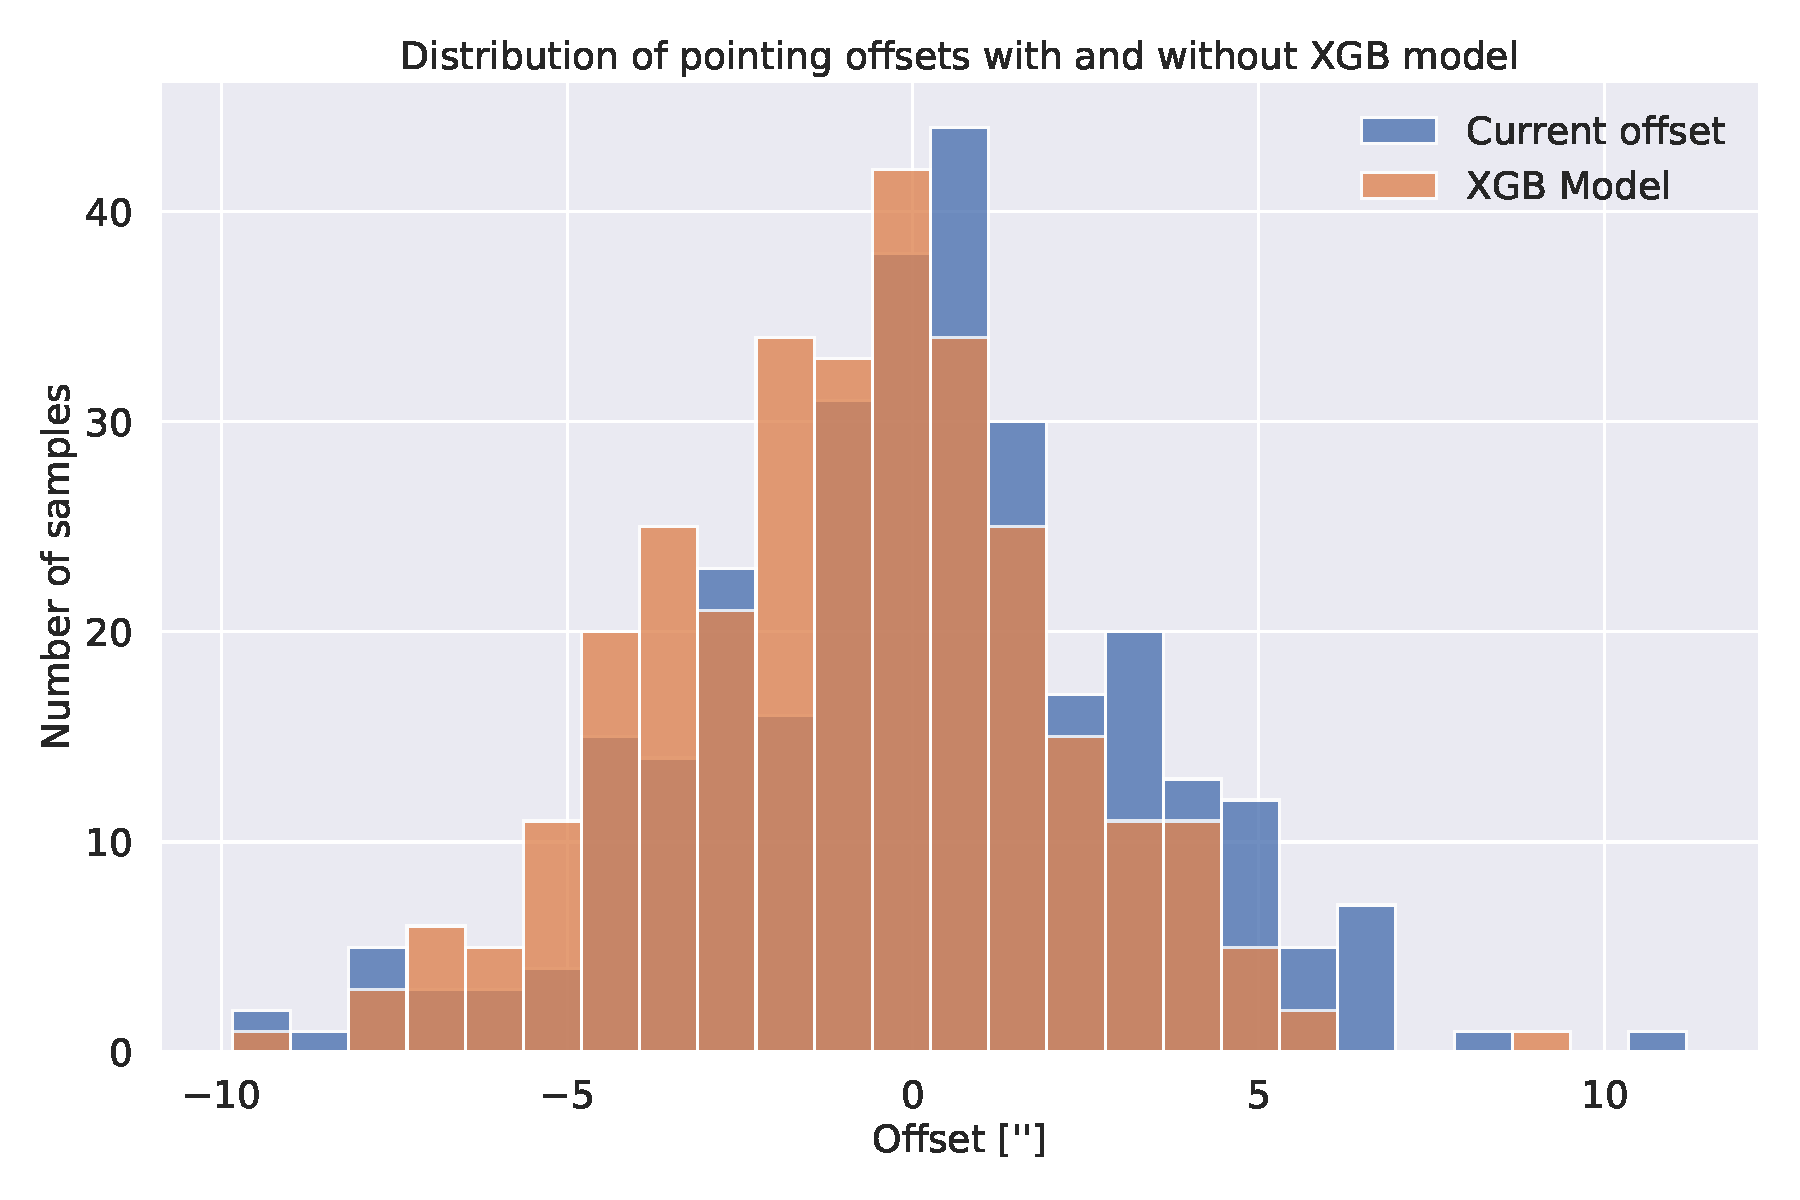
\includegraphics[width=\textwidth]{Results/hist_XGB_ds2_tp5_k30_uncorr_az_test.pdf}
        \caption{NFLASH230 elevation model}
        \label{subfig:hist_lastfold_nflash230_az}
    \end{subfigure}
    \\
    \begin{subfigure}[t]{\textwidth}
       \centering
       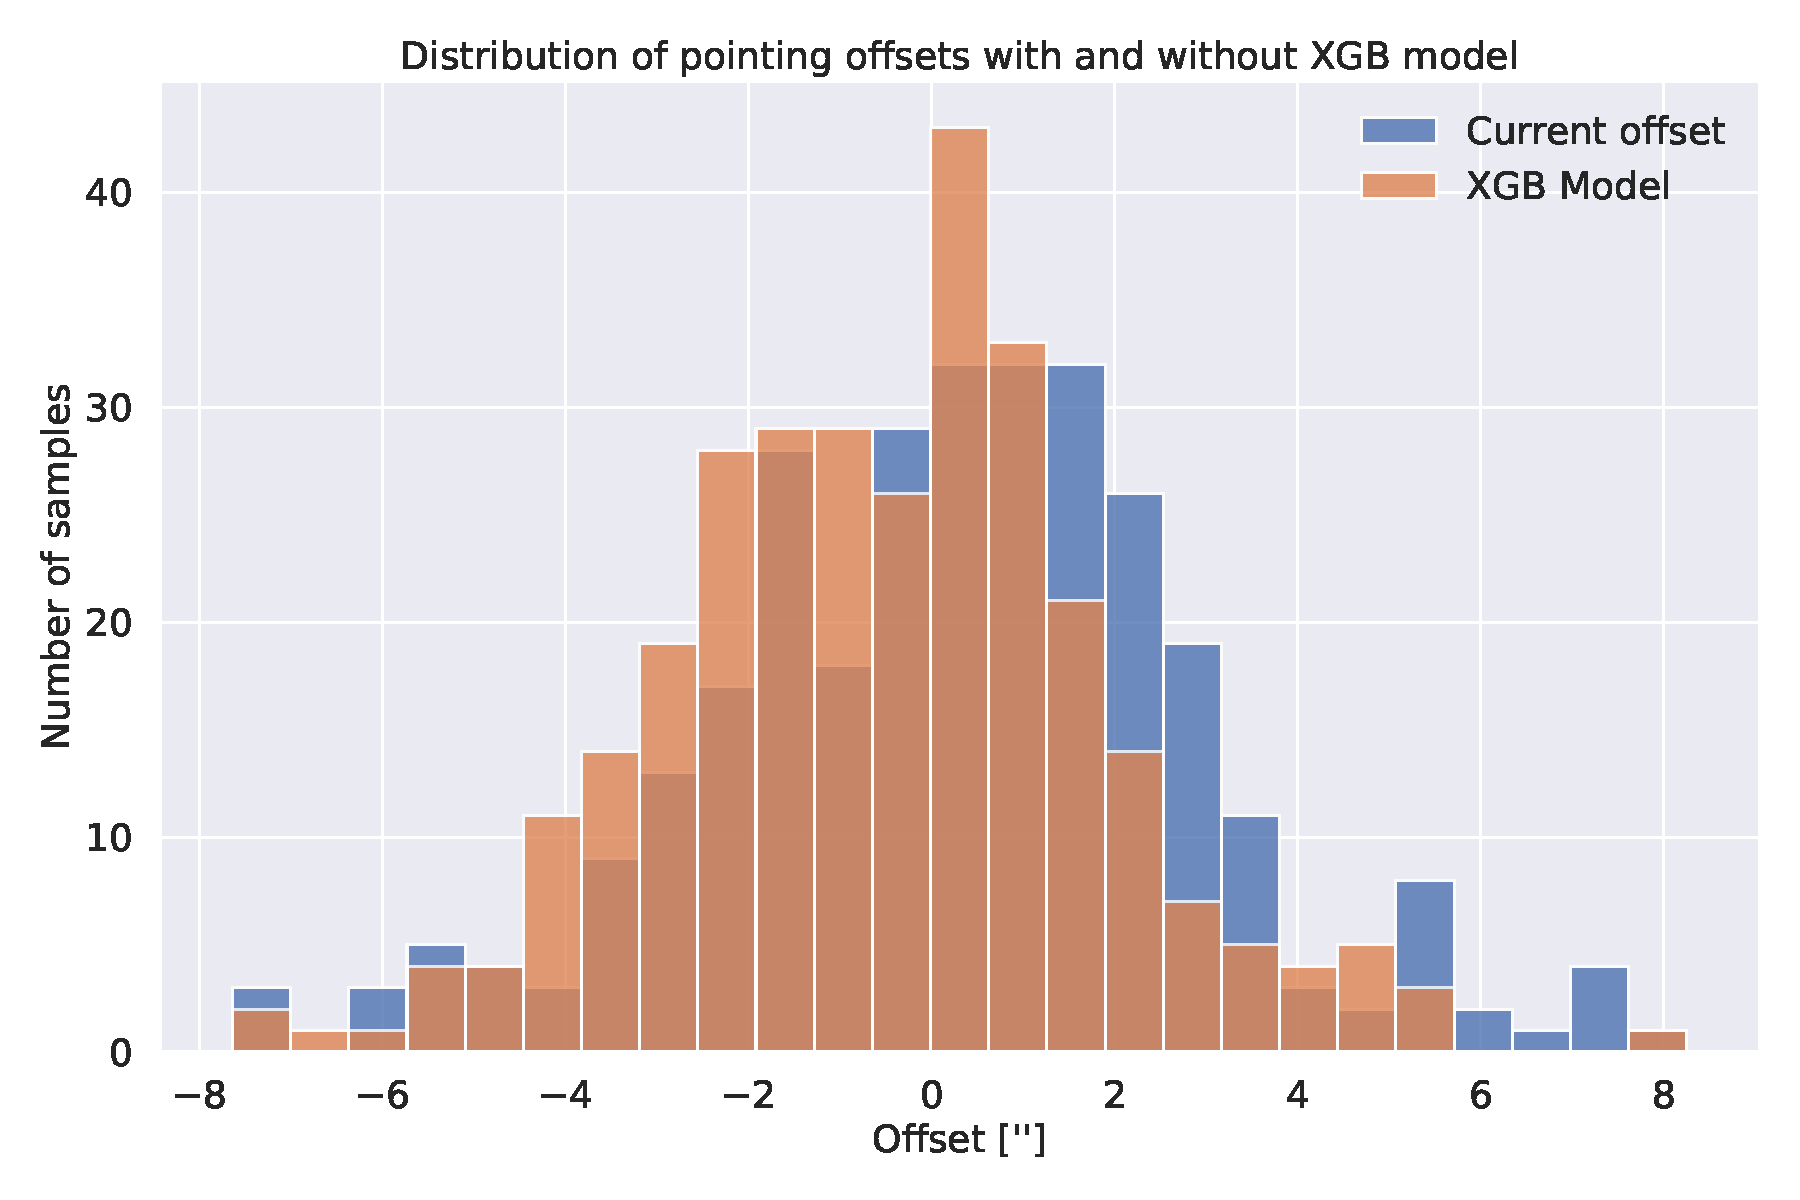
\includegraphics[width=\textwidth]{Results/hist_XGB_ds2_tp5_k40_uncorr_el_test.pdf}
       \caption{NFLASH230 elevation model}
       \label{subfig:hist_lastfold_nflash230_el}
    \end{subfigure}
    \caption{Distribution of offsets with and without XGBoost NFLASH230 pointing correction model}
    \label{fig:histogram_selected_result_xgb}
\end{figure}


\begin{figure}[H]
    \centering
    \begin{subfigure}[t]{\textwidth}
        \centering
        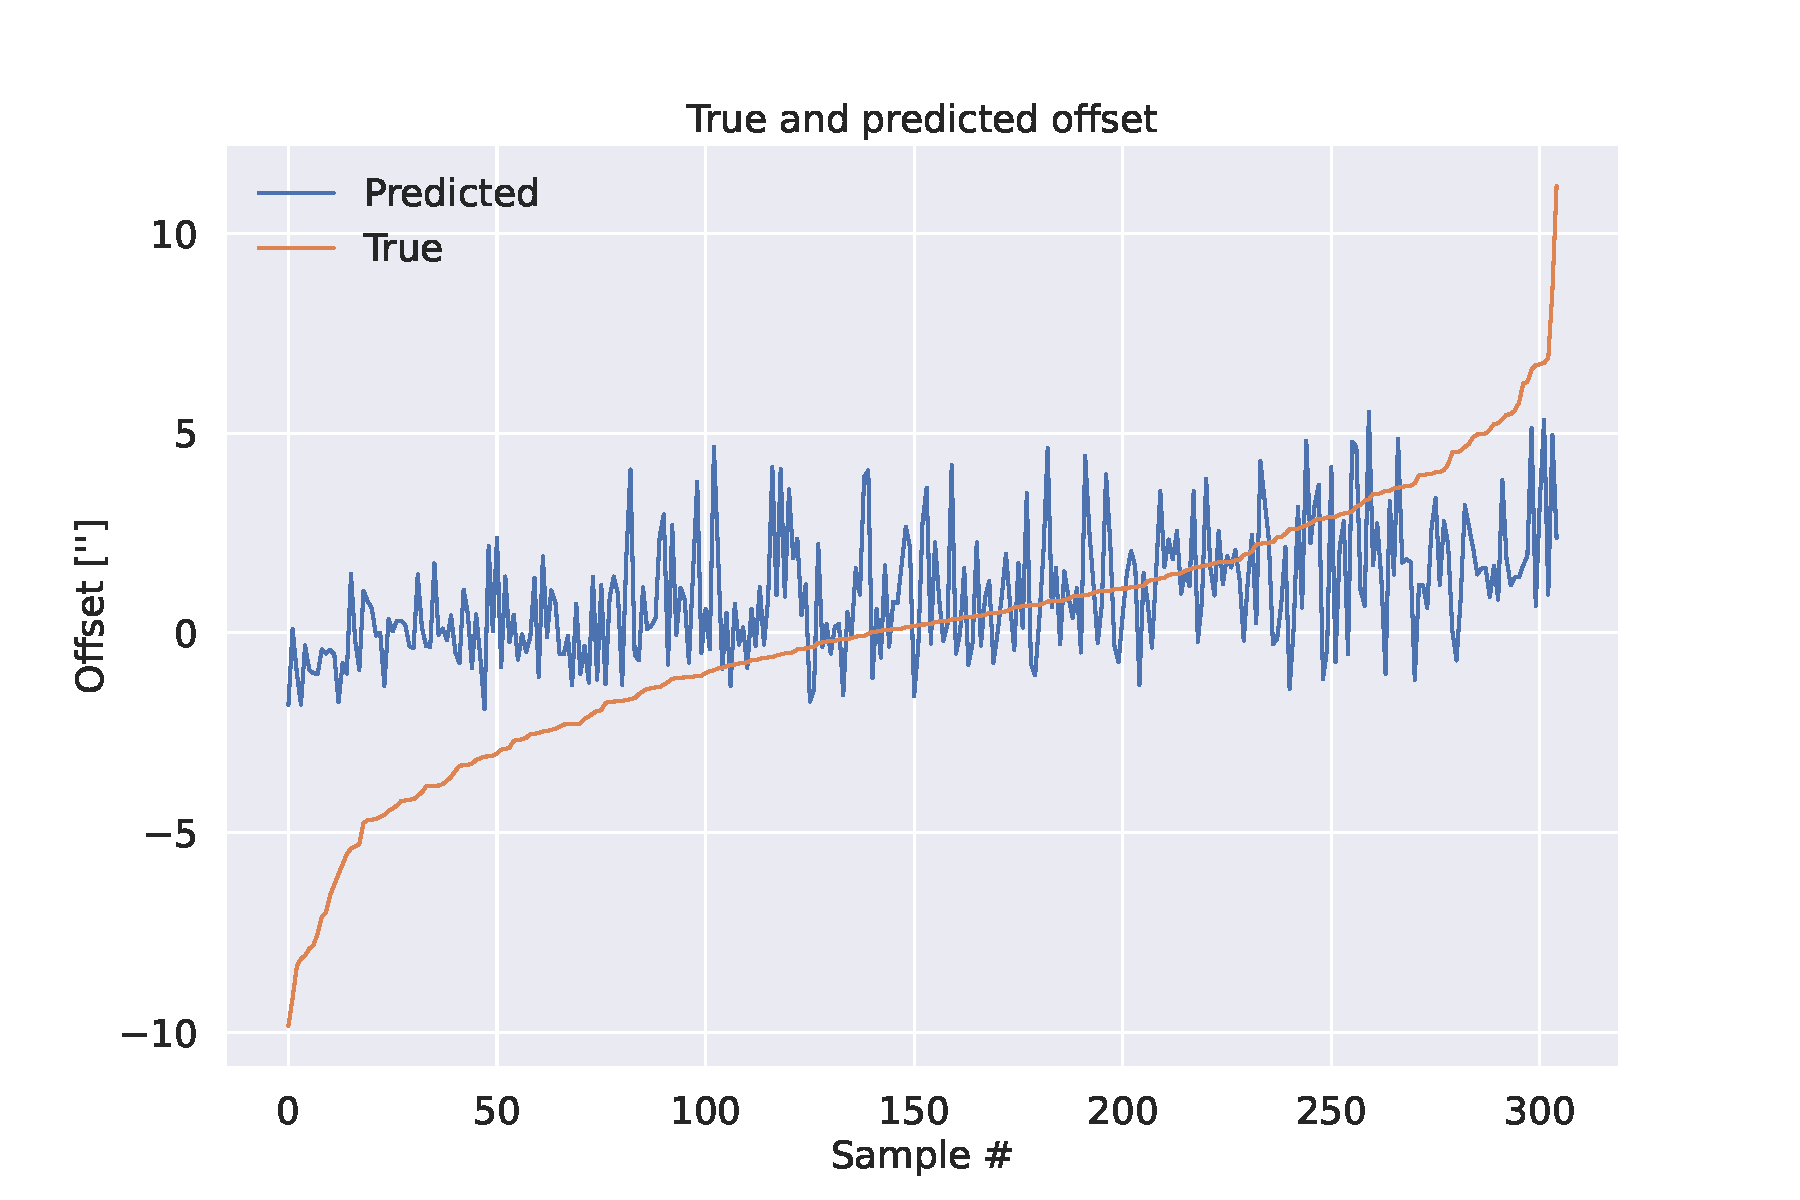
\includegraphics[width=\textwidth]{Results/sortpred_XGB_ds2_tp5_k30_uncorr_az_test.pdf}
        \caption{NFLASH230 azimuth model}
        \label{subfig:sortpred_lastfold_nflash230_az}
    \end{subfigure}
    \\
    \begin{subfigure}[t]{\textwidth}
       \centering
       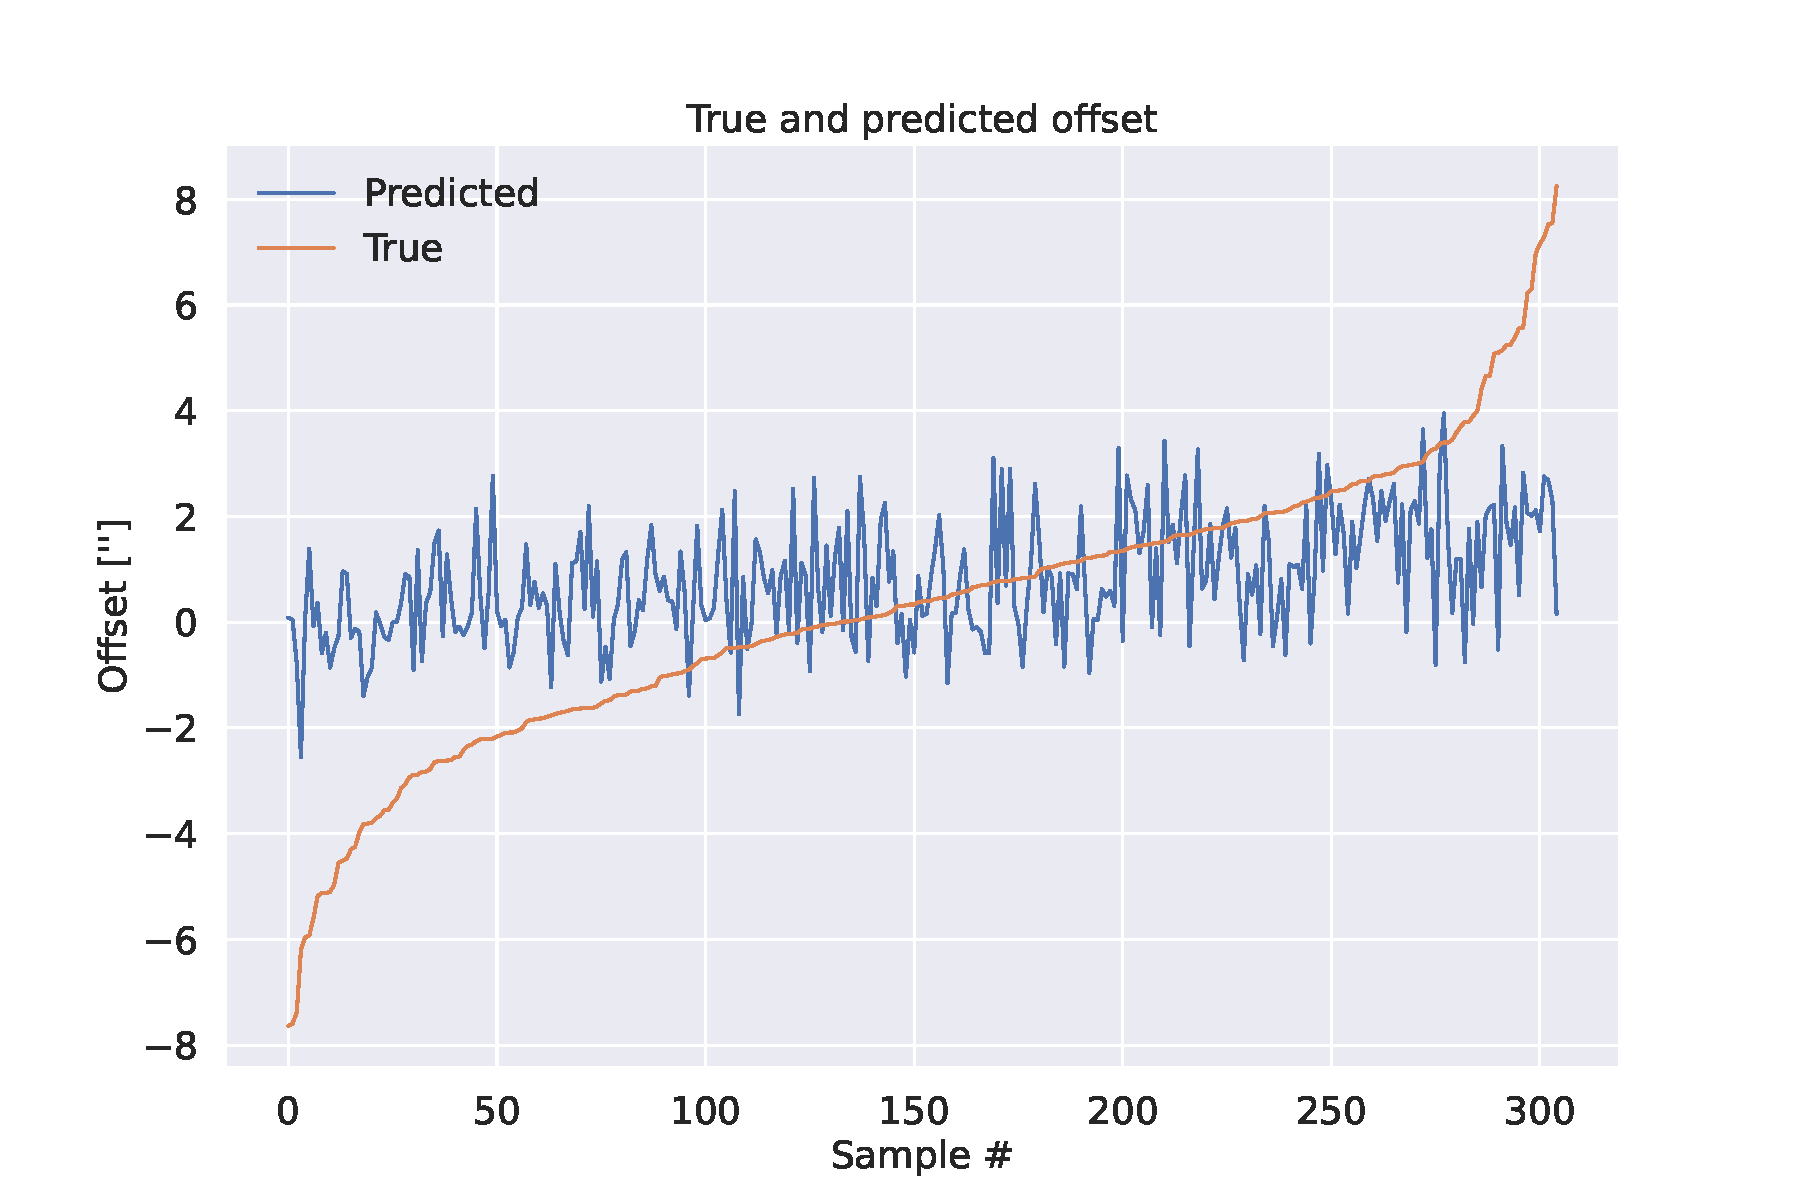
\includegraphics[width=1\textwidth]{Results/sortpred_XGB_ds2_tp5_k40_uncorr_el_test.pdf}
       \caption{NFLASH230 elevation model}
       \label{subfig:sortpred_lastfold_nflash230_el}
    \end{subfigure}
    \caption{Offset predictions by the XGBoost NFLASH230 pointing correction model. Predicted and observed values, sorted in ascending order by observed value}
    \label{fig:sortpred_selected_result_xgb}
\end{figure}


\begin{figure}[H]
    \centering
    \begin{subfigure}[t]{0.92\textwidth}
        \centering
        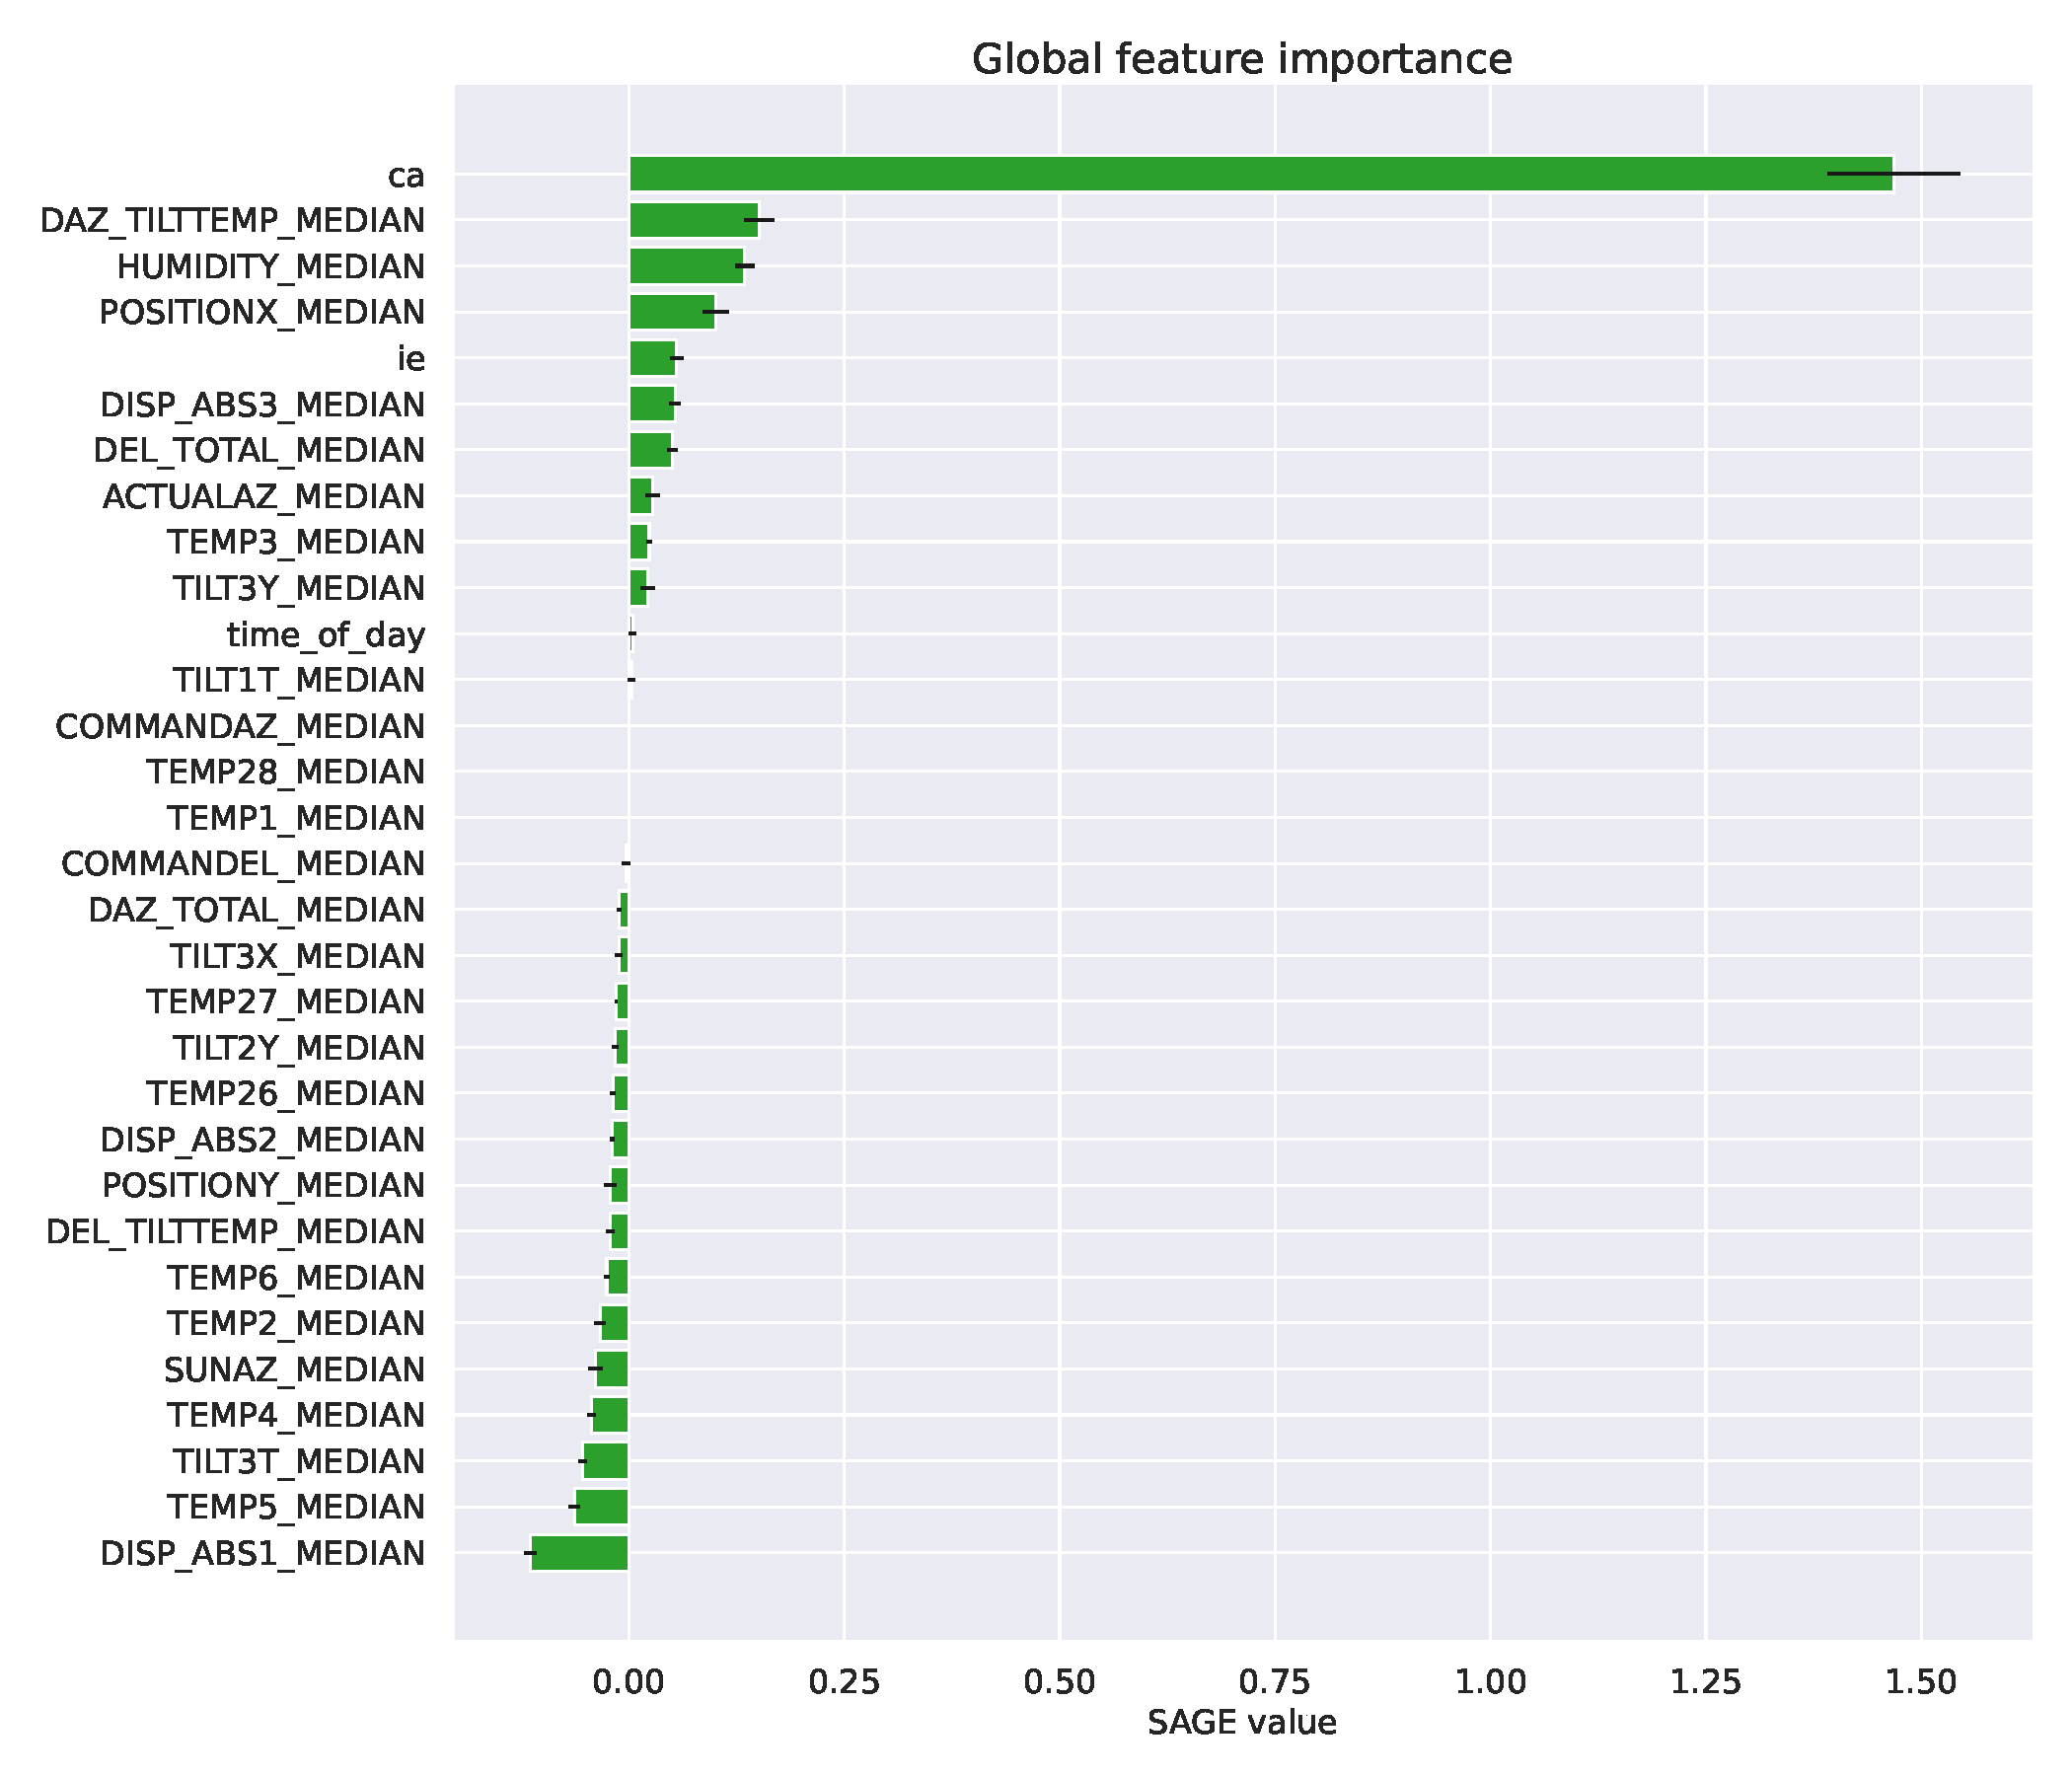
\includegraphics[width=\textwidth]{Results/XGB_ds2_tp5_k30_uncorr_az_val_SAGE.pdf}
        \caption{Validation set}
        \label{subfig:sage_lastfold_nflash230_az_val}
    \end{subfigure}
    \\
    \begin{subfigure}[t]{0.92\textwidth}
       \centering
       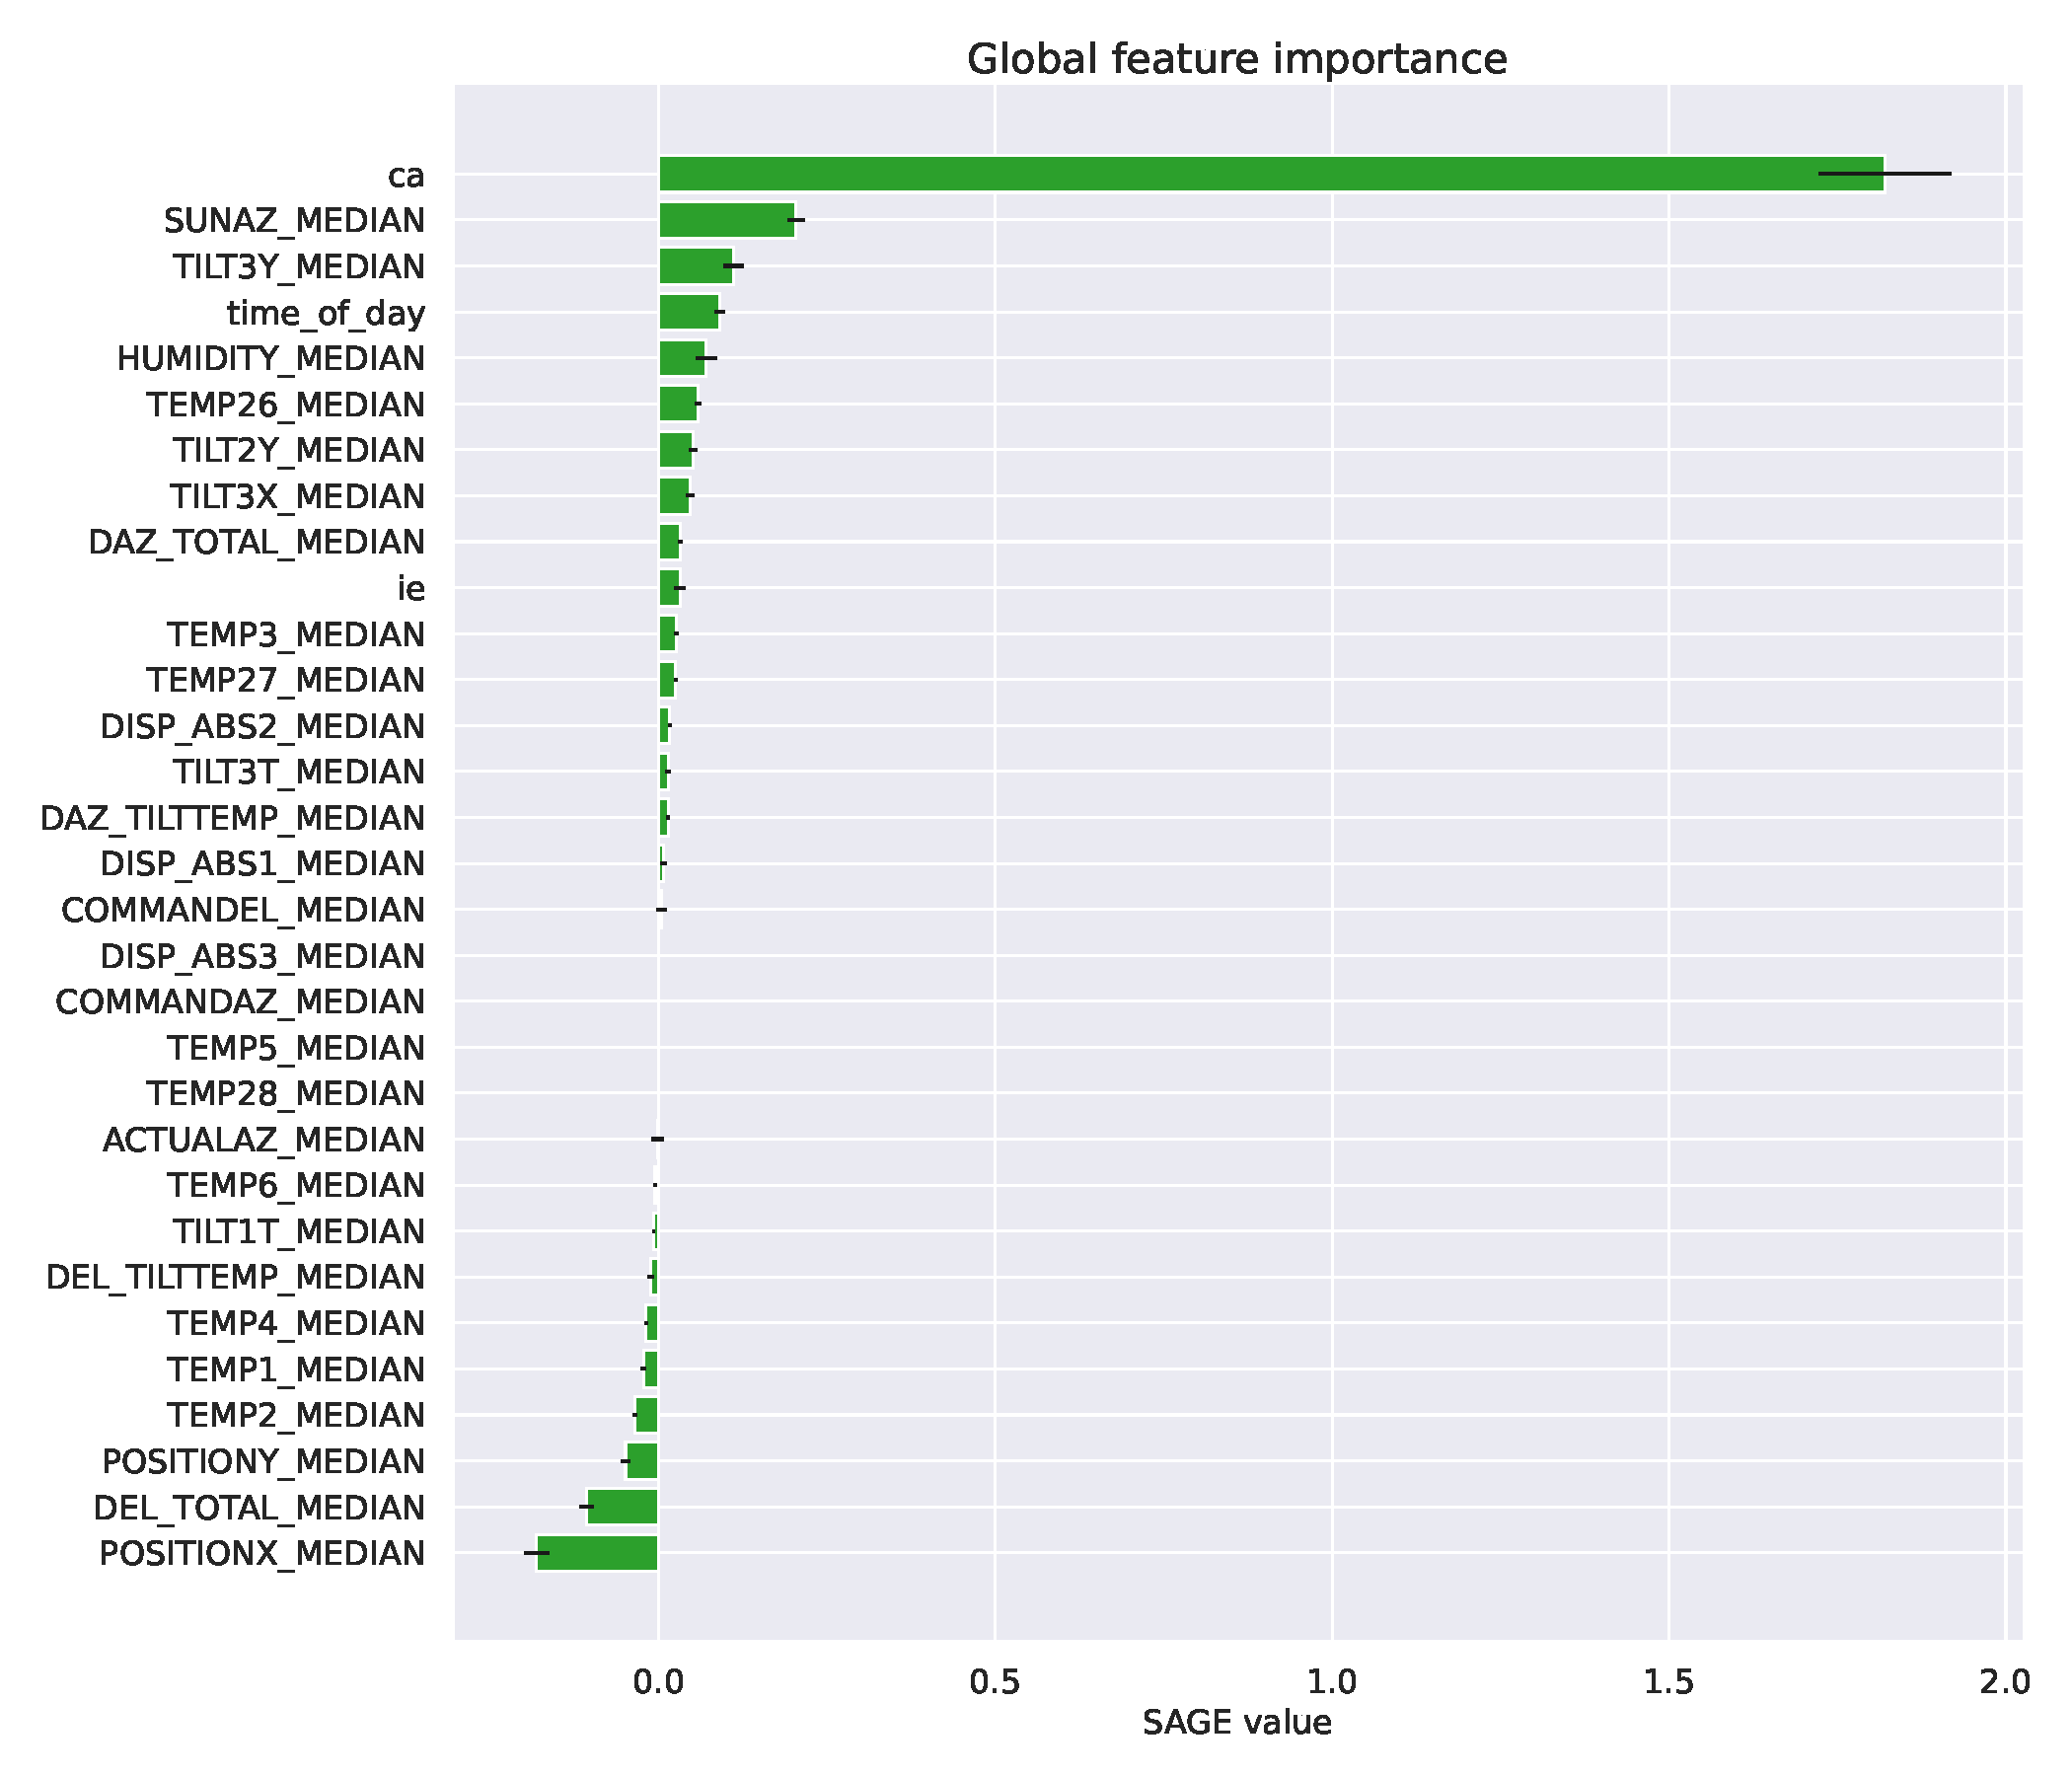
\includegraphics[width=1\textwidth]{Results/XGB_ds2_tp5_k30_uncorr_az_test_SAGE.pdf}
       \caption{Test set}
       \label{subfig:sage_lastfold_nflash230_az_test}
    \end{subfigure}
    \caption{SAGE values for the NFLASH230 azimuth pointing correction model on the a) validation set, and b) test set.}
    \label{fig:sage_lastfold_nflash230_az}
\end{figure}

\begin{figure}[H]
    \centering
    \begin{subfigure}[t]{0.92\textwidth}
        \centering
        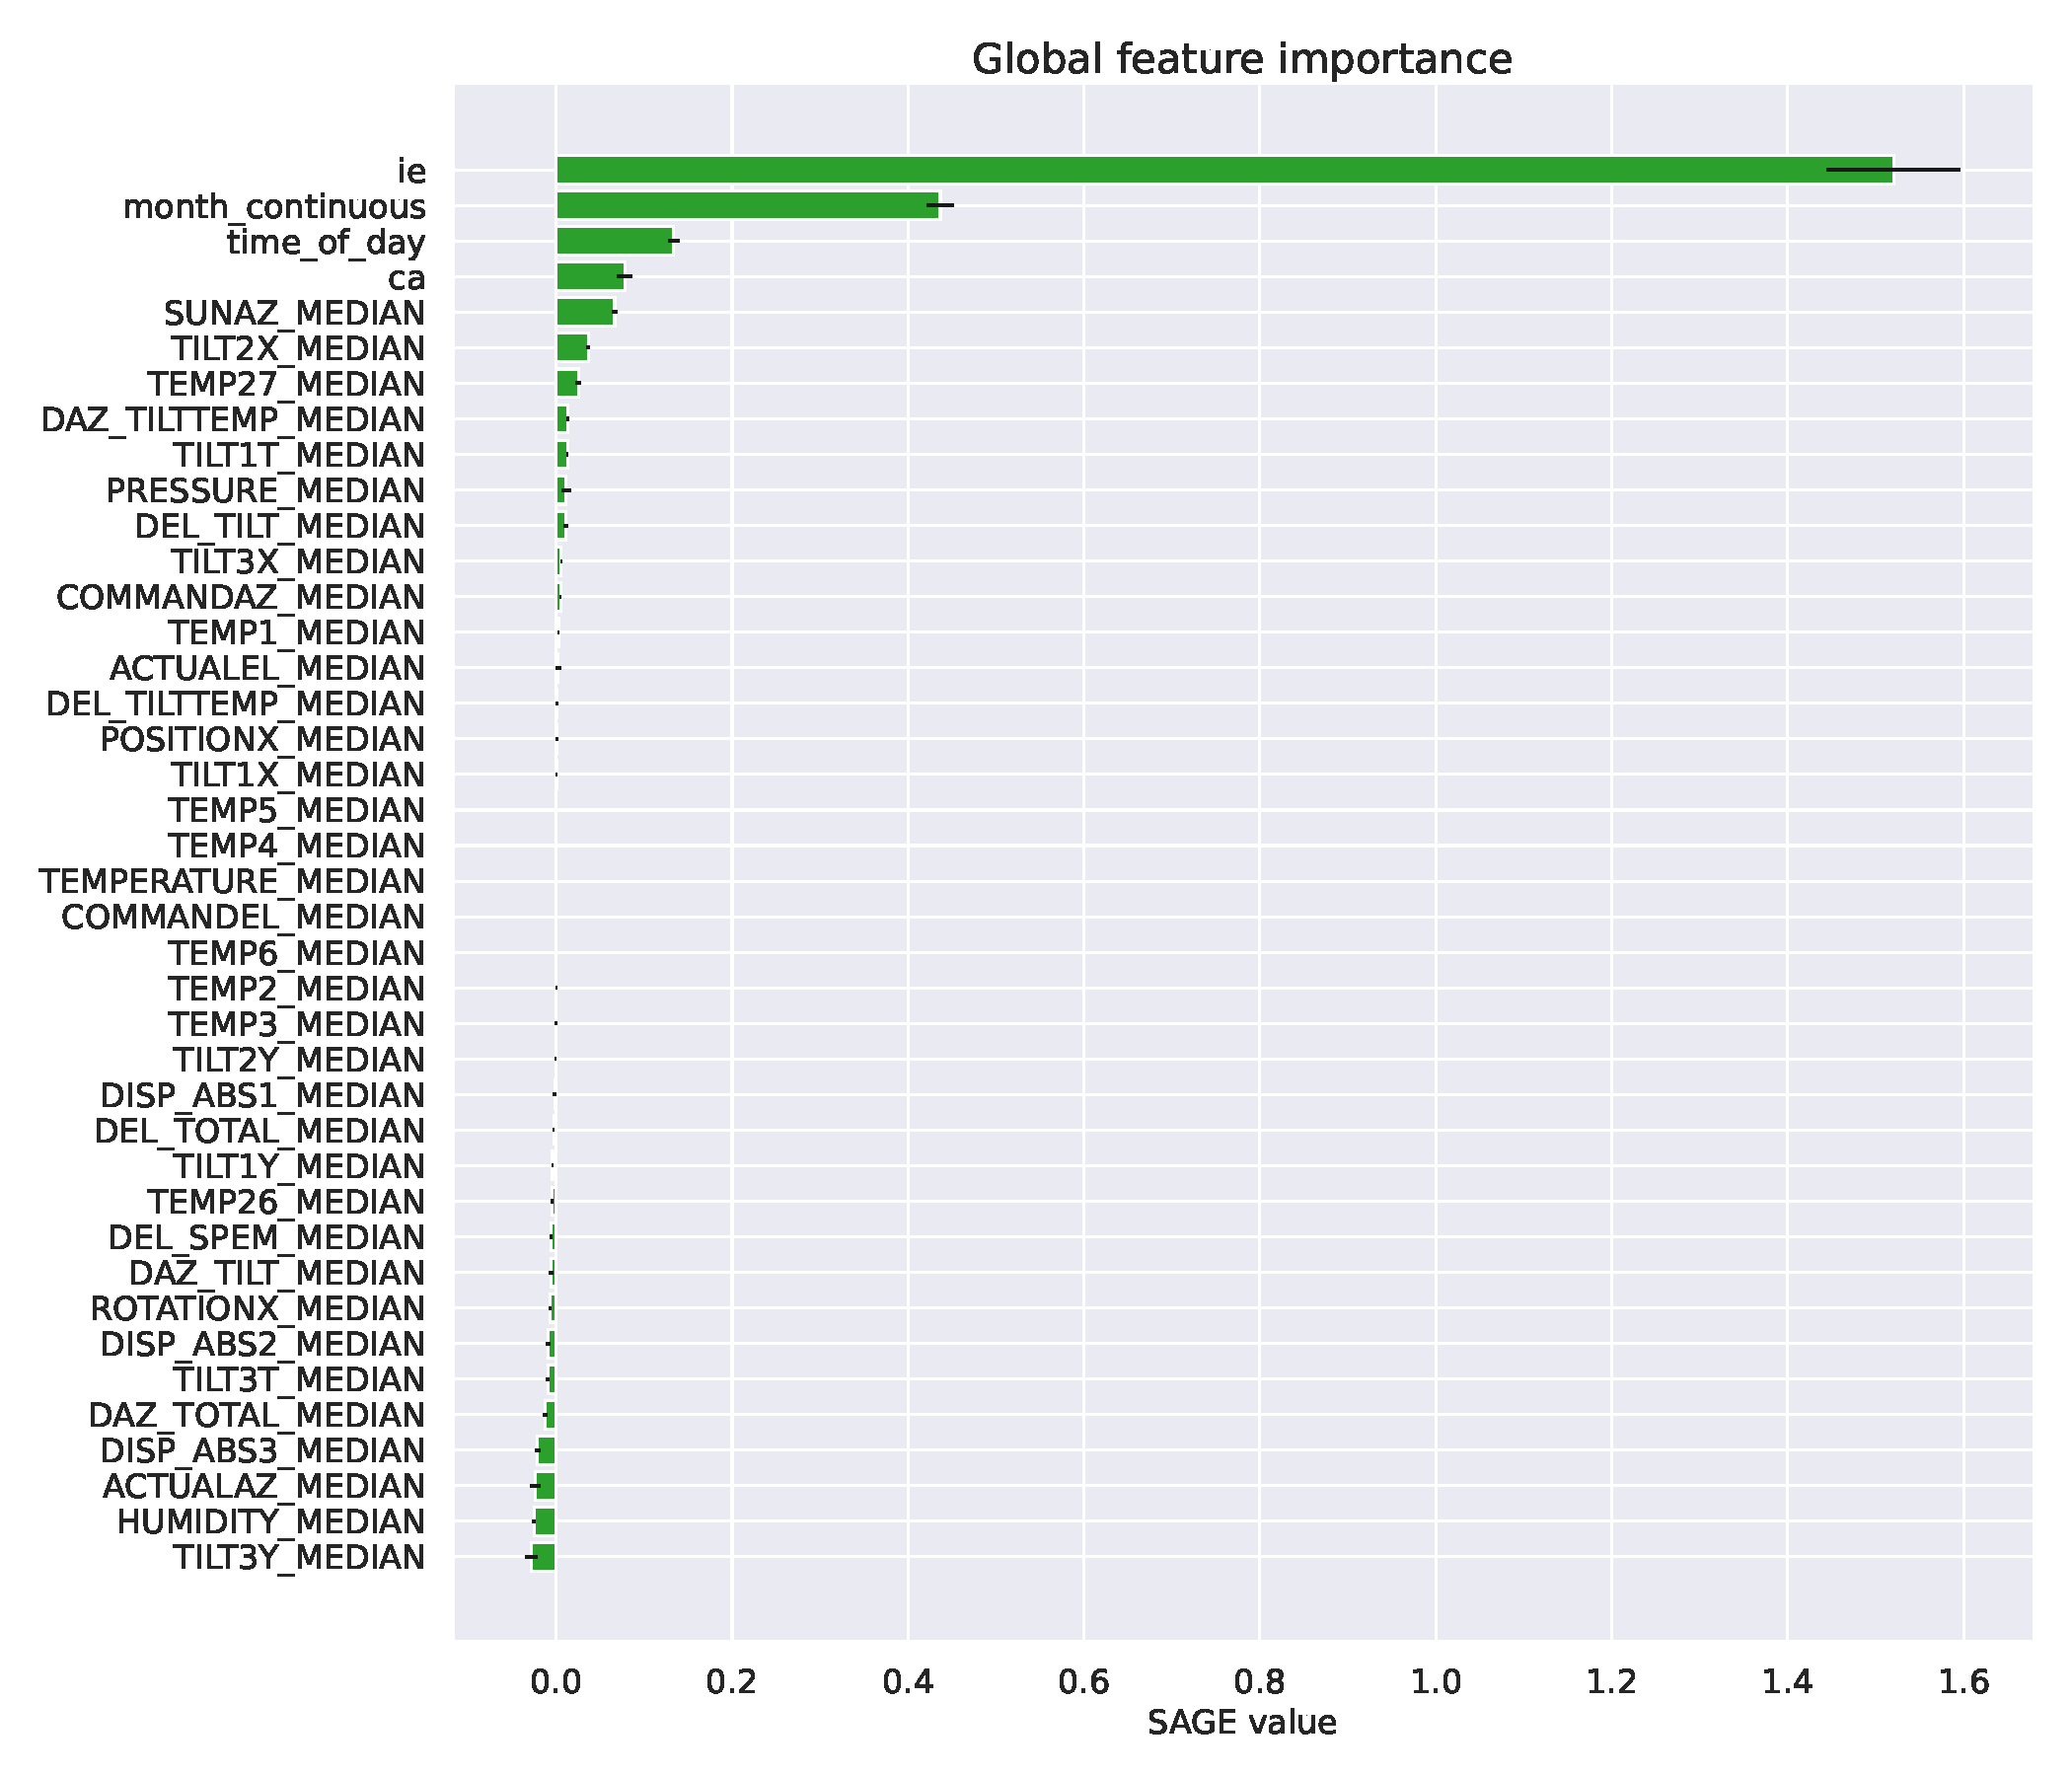
\includegraphics[width=\textwidth]{Results/XGB_ds2_tp5_k40_uncorr_el_val_SAGE.pdf}
        \caption{Validation set}
        \label{subfig:sage_lastfold_nflash230_el_val}
    \end{subfigure}
    \\
    \begin{subfigure}[t]{0.92\textwidth}
       \centering
       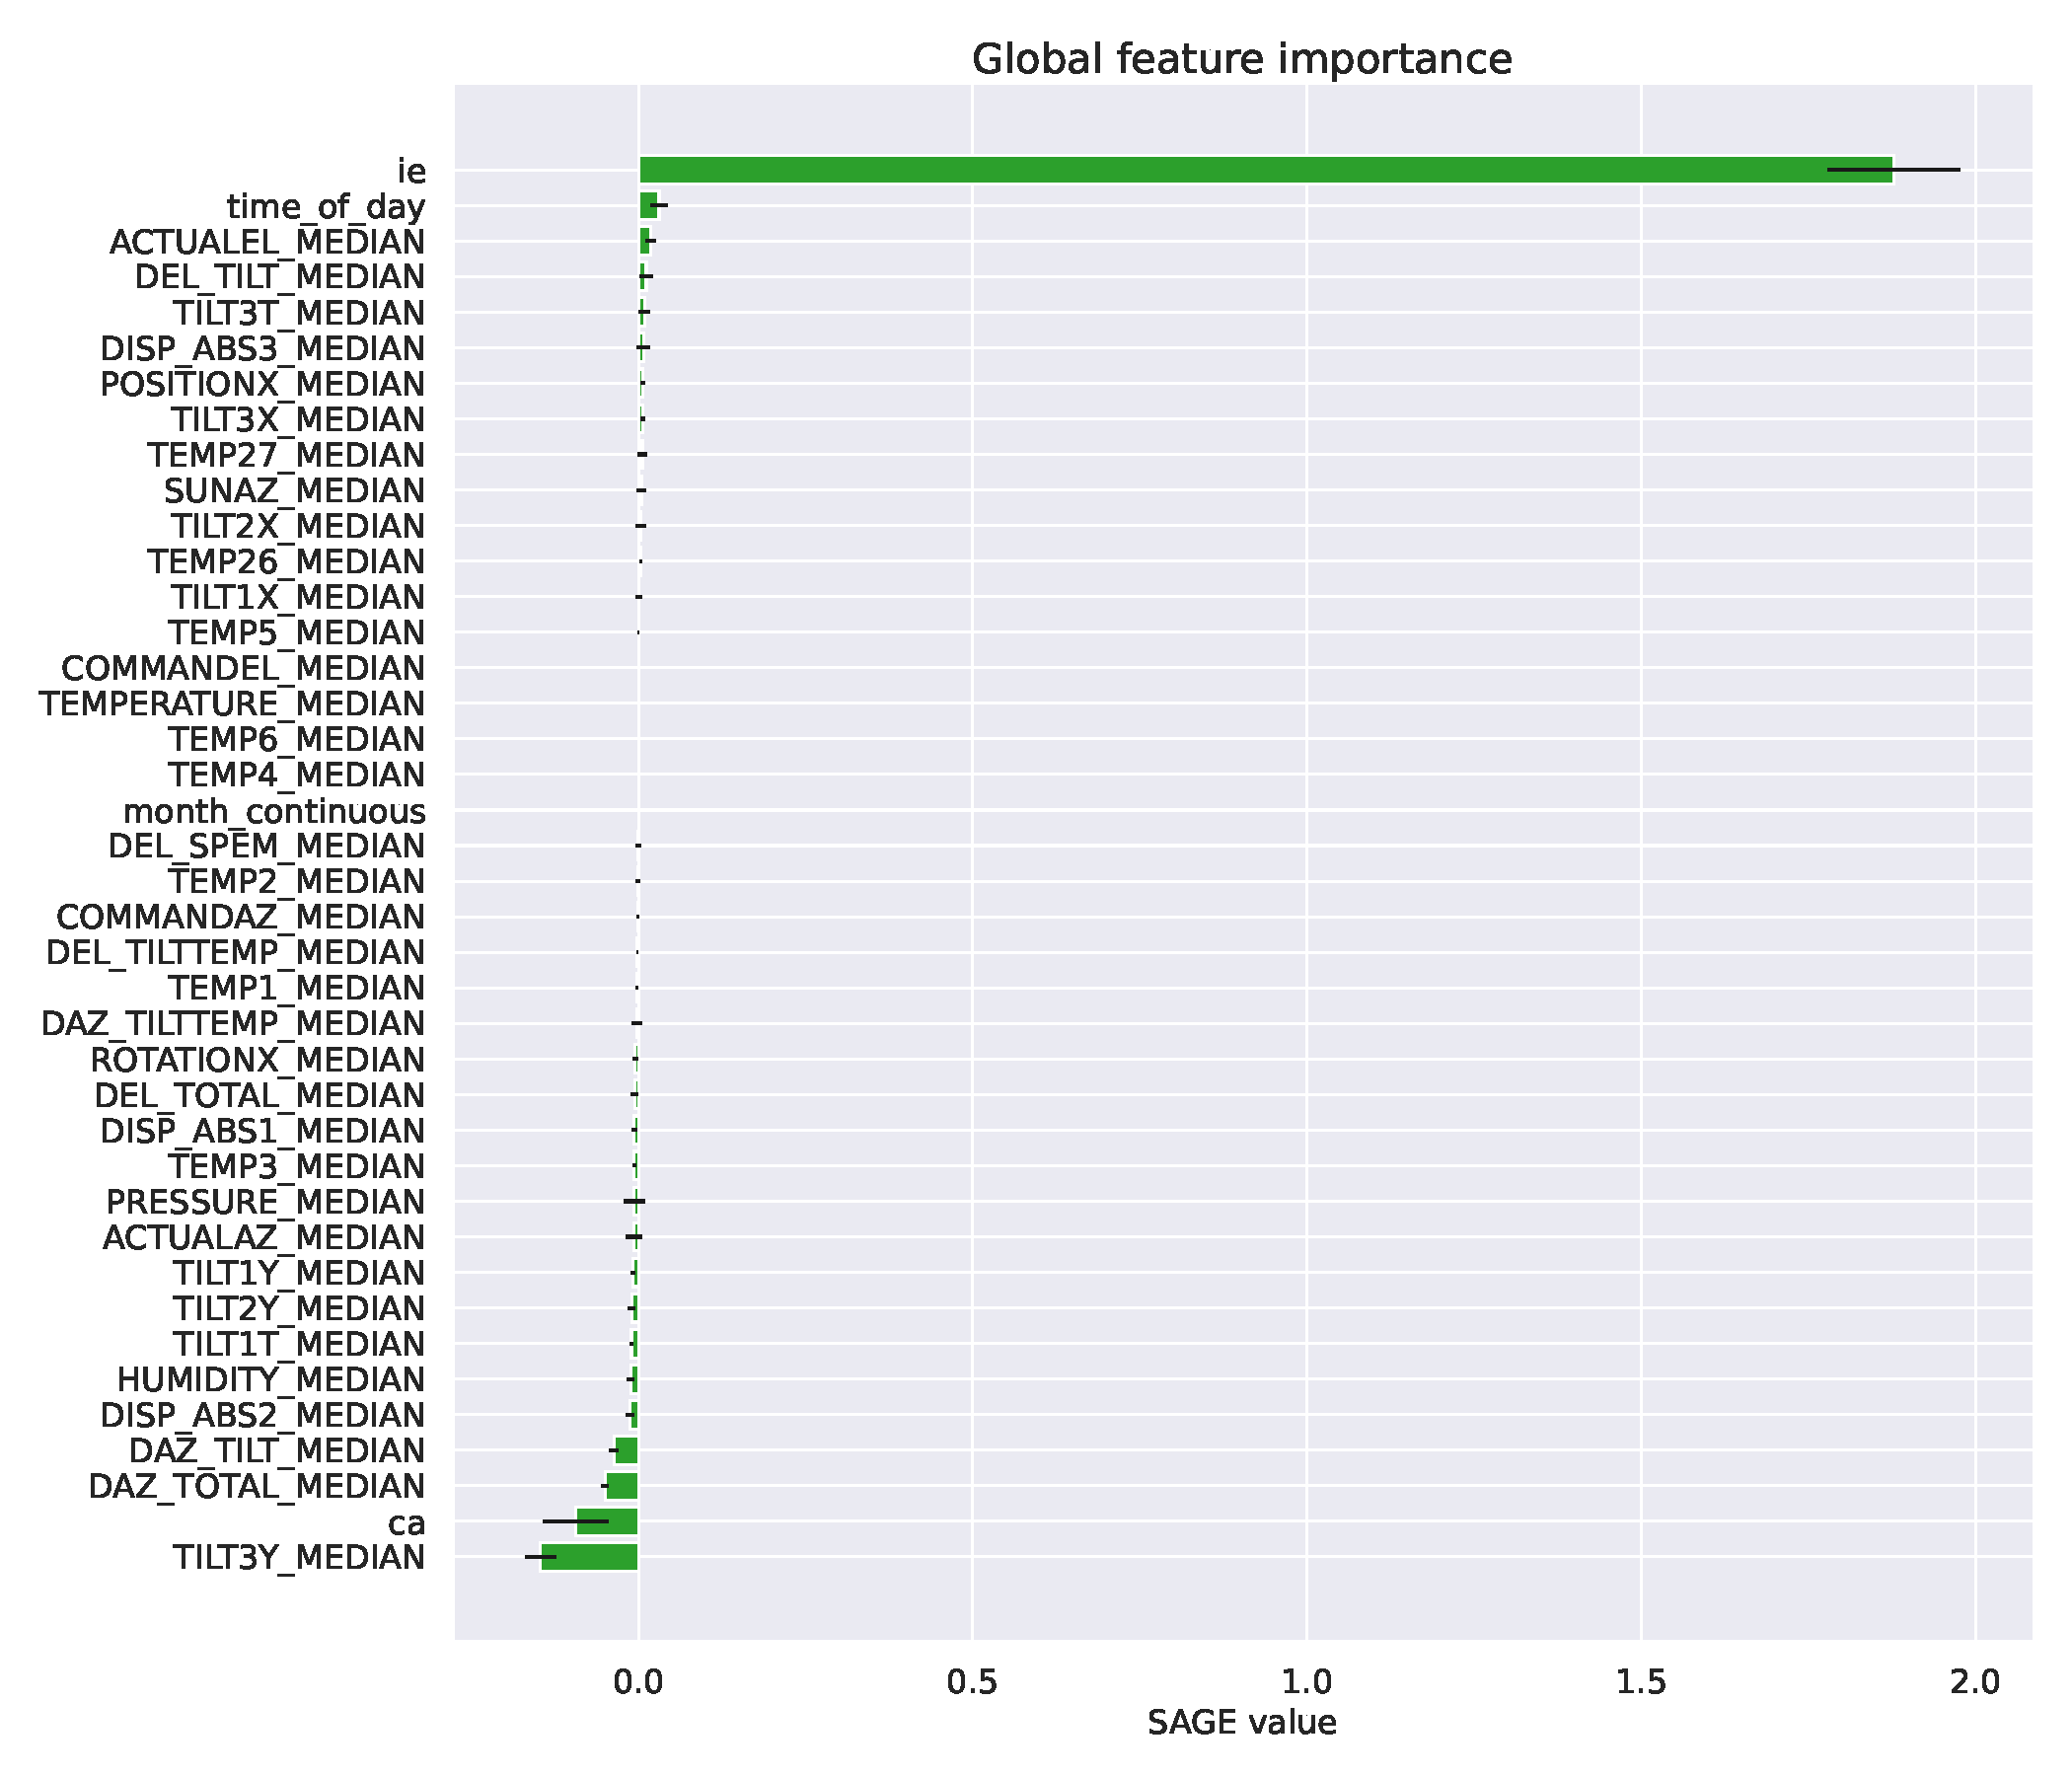
\includegraphics[width=1\textwidth]{Results/XGB_ds2_tp5_k40_uncorr_el_test_SAGE.pdf}
       \caption{Test set}
       \label{subfig:sage_lastfold_nflash230_el_test}
    \end{subfigure}
    \caption{SAGE values for the NFLASH230 elevation pointing correction model on the a) validation set, and b) test set.}
    \label{fig:sage_lastfold_nflash230_el}
\end{figure}





\section{Experiment 2: Pointing Model using Neural Networks}

Table \ref{tab:exp1_rms_folds_best_model} show the RMS in arcseconds on the test set over all folds for the different model arcitechtures.
The models presented in this table are the ones with the lowest mean RMS across all test folds.
A linear regression model is included for comparison. 
It is clear that neural network architectures significantly outperform the linear regressiom model.
From the mean RMS over all folds, we see that the different neural network arcitechtures offer similar performance.
We also see that the RMS of fold $1$ is by far worse than the other folds.
The lowest mean RMS is from the architecture where the non-linear features are connected to the geometrical and harmonic features.\\

\begin{table}[!htbp]
    \centering
    \caption{RMS on all folds for the best model for all arcitechtures. The different arcitechtures are desribed in Figure \ref{fig:nn_architecture}.}
    \begin{tabular}{lcccccccc}
        \toprule
        & \multicolumn{6}{c}{RMS [$''$] on test fold} & & \\
        \cmidrule(lr){2-7}
        Network & 1 & 2 & 3 & 4 & 5 & 6 & Mean & STD\\
        \midrule
        Regular           & 28.06 & 19.34 & 12.28 & 13.25 & 17.19 & 16.33 & 17.74 & 5.19 \\
        Seperated 1       & 30.69 & 16.93 & 13.76 & 10.04 & 15.77 & 13.61 & 16.80 & 6.57 \\
        Seperated 2       & 27.34 & 20.75 & 12.65 & 24.17 & 13.64 & 16.69 & 19.21 & 5.38 \\
        Seperated 3       & 30.27 & 20.59 & 14.01 & 10.76 & 13.67 & 10.34 & 16.61 & 6.97 \\
        Linear regression & 70.55 & 40.19 & 51.17 & 49.69 & 36.86 & 37.29 & 47.63 & 12.81 \\
        \bottomrule
    \end{tabular}
    \label{tab:exp1_rms_folds_best_model}
\end{table}


Table \ref{tab:exp1_hyperparameters_best_model} show the hyperparameter used for the best models.
All arcitechtures perform better with a single hidden layer.
The regular neural network uses ReLU activation and MSE loss, while the other arcitechtures use Tanh activation and MSD loss.
The regular neural network also have more neurons in the hidden layer and a higher learning rate.
The batch size is also varying. There seem to be some similarities between the hyperaprameters chosen for the three arcitectures with seperate features.
However, given the large standard deviation of the mean RMS, there is probably bigger issues than hyperparameter tuning.\\

\begin{table}[!htbp]
    \centering
    \caption{Hyperparameters used in the best performing model for each arcitechture.}
    \begin{tabular}{lccccc}
        \toprule
        Architecture & Activation & Hidden Layers & Learning Rate & Batch Size & Loss \\
        \midrule
        Regular &  ReLU & [82] & 0.0199 & 334 & MSE \\
        Sep1    &  Tanh & [40] & 0.0098 & 101 & MSD \\
        Sep2    &  Tanh & [40] & 0.0098 & 101 & MSD \\
        Sep3    &  Tanh & [26] & 0.0039 & 358 & MSD \\
        \bottomrule
    \end{tabular}
    \label{tab:exp1_hyperparameters_best_model}
\end{table}



Table \ref{tab:exp1_features} lists the features selected for the best performing models.


\begin{table}[!htbp]
    \centering
    \caption{Features used in the best performing model for each arcitechture.}
    \begin{tabular}{|l|ccccc|}
        \hline
        Feature & Sep 1 & Sep 2 & Sep 3 & Regular & \\ \hline
        COMMANDAZ & x & x & x & x & \\ \hline
        COMMANDEL & x & x & x & x & \\ \hline
        DISP ABS3 & x & x & x & x & \\ \hline
        CA & x & x & x & & \\ \hline
        NPAE & x & x & x & & \\ \hline
        Constant & x & x & x & & \\ \hline
        $\cos{(\text{COMMANDEL})}$ & x & x & x & & \\ \hline
        $\cos{(2\cdot \text{COMMANDEL})}$ & x & x & x & & \\ \hline
        $\cos{(3\cdot \text{COMMANDEL})}$ & x & x & x & & \\ \hline
        $\cos{(4\cdot \text{COMMANDEL})}$ & x & x & x & & \\ \hline
        $\cos{(5\cdot \text{COMMANDEL})}$ & x & x & x & & \\ \hline
        $\sin{(\text{COMMANDEL})}$ & x & x & x & & \\ \hline
        $\sin{(2 \cdot \text{COMMANDEL})}$ & x & x & x & & \\ \hline
        $\sin{(3 \cdot \text{COMMANDEL})}$ & x & x & x & & \\ \hline
        $\sin{(4 \cdot \text{COMMANDEL})}$ & x & x & x & & \\ \hline
        $\sin{(5 \cdot \text{COMMANDEL})}$ & x & x & x & & \\ \hline
        Turbulence & x & x & x & & \\ \hline
        DEL TILTTEMP & x & x & x & & \\ \hline
        DAZ DISP & & & x & & \\ \hline
        POSITIONY & & & x & & \\ \hline
        TILT1Y & & & x & & \\ \hline
        TEMPERATURE & & & x & & \\ \hline
        TILT1T & & & x & & \\ \hline
    \end{tabular}
    \label{tab:exp1_features}
\end{table}

\newpage



